\documentclass[
  a4paper,            % DIN A4
  DIV=10,             % Schriftgröße und Satzspiegel
  oneside,            % einseitiger Druck
  BCOR=5mm,           % Bindungskorrektur
  parskip=half,       % Halber Abstand zwischen Absätzen
  numbers=noenddot,   % Kein Punkt hinter Kapitelnummern
  bibliography=totoc,  % Literaturverzeichnis im Inhaltsverzeichnis
  listof=totoc,       % Abbildungs- und Tabellenverzeichnis im Inhaltsverzeichnis
  table
]{scrreprt}
\usepackage{../style/thesisstyle}

% ADDITIONAL PACKAGES
\usepackage{listings}
\usepackage{float}

% CUSTOM COMMANDS
\newcommand{\q}[1]{\glqq{}#1\grqq{}}

\makeglossaries           % create all glossary entries (remember: run makeglossaries manually)
\loadglsentries{thesisglossaries.tex}  % load acronym, symbol and glossary entries

% Synonyms START
% Store = State-Manager = State-Management Library
% Library = Bibliothek = Dependency
% Zustand = State = Applikationszustand
% Synonyms END

\sisetup{locale = DE}     % siunitx locale setup
%\DeclareSIUnit \fps{fps}  % a custom unit (usage: \SI{24}{\fps})

\begin{document}
% !TEX root = ../thesis.tex
%
% configurations
%

% English Language support
% -> uncomment if needed
% Beta!
%\fullenglish{yes}
\fullenglish{no}

% text field
%-> replace supervisor names with correct ones
\firstSupervisor{Prof. Dr. Stefan Sarstedt}
\secondSupervisor{Prof. Dr.-Ing. Lars Hamann}

% text field
%-> replace title with your thesis title
\thesisTitle{Erhöhung der Korrektheit des States in Frontend Webapplikationen mit Strikten Übergängen}
% TODO Title knapper schreiben
\thesisTitleEN{Increasing Correctness in State of Frontend Web Applications with Strict Transitions}

% text field
%-> replace the key words with your own key words
\keywordsDE{State-Management, Webapplikationen, Frontend}
\keywordsEN{State Management, Web Applications, Frontend}

% text field
%-> replace the text with a description of the thesis
\abstractDE{Frontend-Applikationen sind ein wesentlicher Bestandteil jeder Webapplikation und sind für Teile der Geschäftslogik und die UI verantwortlich. Steigende Anforderungen in Geschwindigkeit, Responsiveness und Features erhöhen die Komplexität enorm. Um einen Teil dieser Komplexität zu verwalten, kommen \acrlong{ac:sm}-Lösungen zum Einsatz. Diese übernehmen wichtige Aufgaben wie beispielsweise das Data-Fetching, die Datentransformation und die Datenspeicherung. Fehler im State können daher einen verhältnismäßig großen Einfluss auf das Nutzererlebnis und das operative Geschäft haben. Damit Fehler und Defekte in diesem Bereich reduziert und schnell erkannt werden, wird eine strikte Erweiterung für \acrlong{ac:sm} im Allgemeinen vorgestellt und mit dem normalen Ansatz verglichen.}
\abstractEN{Frontend applications are an essential part of any web application and are responsible for parts of the business logic and the UI. Increasing demands for speed, responsiveness, and features significantly raise complexity. To manage part of this complexity, state management solutions are used. These handle important tasks such as data fetching, data transformation, and data storage. Errors in the state can, therefore, have a relatively large impact on the user experience and operational business. To reduce and quickly detect errors and defects in this area, a strict extension for state management, in general, is introduced and compared to the conventional approach. A reduction in error-proneness as well as improvements in developer experience, readability, and maintainability are considered plausible, even though these aspects could not be definitively proven within the scope of the study.}

% text field
%-> replace john with your name
\thesisAuthor{Soheil Nazari}

% text field
%-> enter the submission date
% TODO UPDATE THIS
\submissionDate{03. März 2025}

% switch - uncomment only one
%-> uncomment NDA or public
%\NDA{yes}
\NDA{no}

% switch - uncomment only one
%-> uncomment old standard cover or cover Corporate Design 2017
\Cover{CD2017}
%\Cover{CD2017NoLogo}
%\Cover{Std2018}
%\Cover{Std2018_green} 			% with green bar

% switch - uncomment only one
%-> uncomment to show list of figures or not
\ListOfFigures{yes}
%\ListOfFigures{no}

% switch - uncomment only one
%-> uncomment to show list of tables or not
\ListOfTables{yes}
%\ListOfTables{no}

% switch - uncomment only one
%-> uncomment to show list of accronyms or not
\ListOfAccronyms{yes}
%\ListOfAccronyms{no}

% switch - uncomment only one
%-> uncomment to show list of symbols or not
\ListOfSymbols{yes}
%\ListOfSymbols{no}

% switch - uncomment only one
%-> uncomment to show list of glossary entries or not
\Glossary{yes}
%\Glossary{no}

% switch - uncomment only one
%-> uncomment the study course you are in
%\studycourse{ITS}
%\studycourse{TI}
%\studycourse{AI}
\studycourse{WI}
%\studycourse{EI}
%\studycourse{REE}
%\studycourse{BMP}		
%\studycourse{BMP-hp}	 % Internship Report in M&P
%\studycourse{BMT}
%\studycourse{BMT-st}    % Study / home assignment in BMT
%\studycourse{BMT-hp}    % Internship Report in BMT
%\studycourse{MI}
%\studycourse{MIK}
%\studycourse{MA}
    % load all settings

\hyphenation{Ba-che-lor-the-sis Mas-ter-the-sis}

% Cover page here, no page number
\ICoverPage

% PDF Metadata
% !TEX root = ../thesis.tex
%
% PDF Metadata integration
% @author Thomas Lehmann
%

% PDF Metadata
\hypersetup{
pdftitle={\IthesisTitle},
pdfauthor={\IthesisAuthor},
pdfkeywords={\IkeyWordsEN}
}

% Titlepage is page one even if the number is not shown.
\pagenumbering{roman}
% Title page here
% !TEX root = ../thesis.tex
%
% title page
% @author Thomas Lehmann
% Hints for title page and page numbering: https://en.wikipedia.org/wiki/Title_page
%
\title{\IthesisTitle}   % set latex default title to be used by hyperref in pdf
\author{\IthesisAuthor} % set latex default author to be used by hyperref in pdf

\newpage
\thispagestyle{empty}
{\fontfamily{phv}\selectfont
  \hfuzz=20pt       % suppress warnings due to extension onto page margins

  % Author of thesis
  \vspace*{1cm}
  \begin{minipage}[b]{\textwidth}
    \fontsize{14pt}{20pt}
    \selectfont
    \begin{center}
      \IthesisAuthor
    \end{center}
  \end{minipage}

  % Title of thesis
  \vspace{1.5cm}
  \begin{minipage}[b][0cm][t]{\textwidth}
    \fontsize{18pt}{20pt}
    \selectfont
    \begin{center}
      \IthesisTitle
    \end{center}
  \end{minipage}

  % Important information
  \begin{textblock*}{\textwidth}(40mm,210mm)
    \begin{minipage}[b]{\textwidth}
      \hbadness=10001    % suppress underfull warning due to short text
      \fontfamily{cmr}\selectfont
      \fontsize{12pt}{14pt}
      \selectfont
      \ifdefined\ILanguageEN
        \IthesisKindEN ~submitted for examination in \IthesisExaminationEN \\
        in the study course \textit{\IstudyCourseName} \\
        at the \IthesisDepartmentFullEN \\
        at the \IthesisFacultyFullEN \\
        at University of Applied Science Hamburg\\

        Supervisor: \IfirstSv \\
        \ifdefined\IisTermPaper
          % left blank
        \else
          \ifdefined\IisInternshipReport
	  Supervised: \IsecondSv\\
          \else
        Supervisor: \IsecondSv \\
          \fi\fi
        
        Submitted on: \ISubDate \\
      \else
      	\ifdefined\IisInternshipReport
        \IthesisKindDE ~eingereicht im Rahmen des \IthesisExaminationDE \\	
	\else
        \IthesisKindDE ~eingereicht im Rahmen der \IthesisExaminationDE \\
        \fi
	im Studiengang \textit{\IstudyCourseName} \\
        am \IthesisDepartmentFull \\
        der \IthesisFacultyFull \\
        der Hochschule für Angewandte Wissenschaften Hamburg\\

        Betreuender Prüfer: \IfirstSv \\
        \ifdefined\IisTermPaper
          % left blank
        \else
          \ifdefined\IisInternshipReport
        betriebliche Betreuung: \IsecondSv \\							
	  \else
        Zweitgutachter: \IsecondSv \\
        \fi\fi

        Eingereicht am: \ISubDate \\
      \fi
    \end{minipage}
  \end{textblock*}
}


% Abstract page here
% !TEX root = ../thesis.tex
%
% abstract page
% @author Thomas Lehmann
%
\newpage
\thispagestyle{plain}
\clearpage
\hfuzz=12pt       % suppress warnings due to extenstion onto page margins

\textbf{\IthesisAuthor}

\vspace{0.3cm}
\textbf{Thema der Arbeit}

\IthesisTitle

\vspace{0.3cm}
\textbf{Stichworte}

\IkeyWordsDE

\vspace{0.3cm}
\textbf{Kurzzusammenfassung}

\begin{minipage}{\textwidth}
\IabstractDE
\end{minipage}

\vspace{1.0cm}
\textbf{\IthesisAuthor}

\vspace{0.3cm}
\textbf{Title of Thesis}

\IthesisTitleEN

\vspace{0.3cm}
\textbf{Keywords}

\begin{minipage}{\textwidth}
\IkeyWordsEN
\end{minipage}

\vspace{0.3cm}
\textbf{Abstract}

\IabstractEN


% Table of contents here
\tableofcontents

% List of figures here
\IListOfFigures

% List of tables here
\IListOfTables

% List of accronyms here
\IListOfAccronyms

% List of symbols here
\IListOfSymbols

% Uncomment if list of source code is needed (rarely).
%\lstlistoflistings  % requires package listings, needs to uncommenting of usepackage

% path to the chapters folder is set to find the images used there
\graphicspath{ {./images/} }

% Chapters
\clearpage
\pagenumbering{arabic}
\chapter{Einleitung}

\section{Die Rolle des State-Managements in Frontend Webapplikationen}

Moderne Webapplikationen folgen der Komponenten-Architektur. Verschiedene Komponenten können von den selben Daten abhängig sein. Die Daten werden in der Regel während der Lebensdauer der Browser-Session basierend auf Interaktionen des Benutzers aktualisiert und erweitert. Änderungen in den Daten müssen den betroffenen Komponenten mitgeteilt werden. In einigen Fällen ist die Synchronisierung der Daten im Frontend mit den Daten des Servers erforderlich. Um HTTP Aufrufe zu sparen, können verschiedene Mechanismen, wie beispielsweise Caching oder Debouncing verwendet werden. Diese Faktoren erhöhen, die ohnehin schon hohe Komplexität und Fehleranfälligkeit zusätzlich.

Um diese Komplexität effizient zu verwalten, werden State-Management Lösungen wie Redux \cite{redux}, NgRx \cite{ngrx} oder Pinia \cite{pinia} verwendet. Mit Hilfe dieser Open Source JavaScript Bibliotheken, können Daten beim Bedarf von einer API abgerufen, transformiert und im Speicher gespeichert werden. Die meisten State-Management Bibliotheken sind eng mit einem UI-Framework gekoppelt. \cite{ui-frameworks-and-state-management}. Aus diesem Grund sind sie ein fundamentaler Baustein jeder größeren Frontend Webapplikation.

\section{Ziel dieser Arbeit}

Mit der Komplexität erhöht sich auch die Fehleranfälligkeit. Fehler im Zustand, also Daten der Applikation, haben einen direkten Einfluss auf das Angezeigte. Wenn die Applikation sich in einem "falschen" Zustand befindet und es keine Laufzeitfehler gab, können die Verantwortlichen (in der Regel, die Entwickler) unter Umständen, nicht darüber informiert sein. Dies führt zu langlebigen Bugs.

Ziel dieser Arbeit ist es, einen Ansatz zu erarbeiten, bei dem die Möglichkeit eines Befindens in einem "falschen" oder "illegalem" Zustand eliminiert wird. Dazu wird jeder zusammenhänge Teil des Zustands als ein endlicher Automat \cite{fa} abgebildet. Dahingehend wird jede Änderung in diesem Zustand wie ein Übergang bei einem endlichen Automaten behandelt. Es wird vorgeschlagen die beliebten State-Management Lösungen um "strikte" Übergänge, wie bei einem DFA, zu erweitern. Auf diesem Wege wird eine Reduzierung von Bugs in größeren Applikationen bestrebt. Dabei wird insbesondere auf die Lesbarkeit und Wartbarkeit des Quellcodes und die Developer Experience geachtet.
\chapter{Methodologie}

TODO 

\section{Code Ausschnitte}

TypeScript wird benutzt um, Aufbau von Objekten oder Funktionen zu beschreiben. Längere Strukturen werden mit Hilfe von Code-Bespielen veranschaulicht. Hierfür wird ebenfalls TypeScript verwendet. An viele Stellen wird auf Type-Annotationen verzichtet, damit die Beispiele leicht lesbar bleiben.
\chapter{State-Management Ansätze} \label{sm-ansaetze}

Bei den populären \acrshort{ac:sm}-Lösungen folgt Redux und NgRx dem Flux-Pattern\cite{historyOfRedux}\cite{ngrxGettingStarted}, wobei Zustand und Pinia einen anderen, Framework-nahen Ansatz verfolgen. Im Folgenden wird die Funktionsweise und die Eigenschaften von Redux und Pinia näher beschrieben. Da diese grundlegend unterschiedliche Ansätze verfolgen und andere \acrshort{ac:sm}-Lösungen sich einem der beiden ähneln.

\section{Redux}

Redux definiert sich durch folgenden vier Eigenschaften:
\begin{enumerate}
  \item Unveränderlichkeit (Immutability): Änderung am State sind ausschließlich über die APIs von Redux unter Beachtung der Unveränderlichkeit möglich.
  \item Zentralisierung des Zustandes: Der gesamte Applikationszustand lebt in einem zentralen \acrlong{ac:js} Objekt.
  \item Nachvollzierbarkeit (Traceability): Während der gesamten Lebensdauer der Applikation, sind Änderungen am Zustand auf deren Ursprung verfolgbar.
  \item Event basiert: Es wird das Beobachter-Muster (Observer Pattern) verwendet.
\end{enumerate}

Das Verhalten des Stores wird durch \textit{actions} und \textit{reducer} definiert.
% Außerdem können optionale \textit{selectors} benutzt werden um aus bestimmten Teilen des Zustandes zu lesen.

\subsection{Actions}

Eine Aktion (Action) beschreibt eine Änderung oder Interaktion in und mit der Applikation. Beispielsweise könnte eine \textit{counter-clicked} Action versendet (dispatch) werden, wenn der Nutzer auf den \textit{Zähler erhöhen} Button drückt. Oder, wenn der Nutzer sich erfolgreich angemeldet hat, kann eine entsprechende Action versendet werden. Intern ist eine Action ein \acrshort{ac:pojo}.\cite{reduxStateActionReducers}

Es wird folgende Struktur für Actions empfohlen:
\begin{lstlisting}
type Action<T> = {
  type: string,
  payload?: T
}
\end{lstlisting}

Das Feld \textit{type} beschreibt die Action und das optionale Feld \textit{payload} enthält weiterführende Daten.

\subsection{Reducer}

Ein Reducer ist für die Initialisierung und Aktualisierung des Zustandes zuständig. Ein Reducer wird als eine Pure-Function mit zwei Parametern definiert.
Der erste Parameter ist das Zustandsobjekt und der zweite die versendete Action. Der Rückgabewert dieser Funktion ist das neue Zustandsobjekt. Da es sich hier um eine Pure-Funtion handelt, dürfen es hier keine Seiteneffekte stattfinden. Wie anfangserwähnt, ist der Zustand Unveränderlich, daher dürfen hier keine direkten Veränderungen des Zustandes stattfinden. Es wird lediglich ein neues Objekt zurückgegeben. Fall es keine Veränderungen stattfinden sollen, kann das ursprüngliche Objekt aus dem ersten Parameter unverändert zurückgegeben werden.\cite{reduxStateActionReducers}

Es wird folgende Struktur für Reducer empfohlen:
\begin{lstlisting}
type Reducer<S, A> = (state: S, action: A) => S
\end{lstlisting}

Beispiel reducer:

\begin{lstlisting}
function reducer(state = { user: null }, action) {
  switch (action.type) {
    case 'user-logged-in':
      return {
        ...state,
        user: {
          userId: action.payload.userId
        },
      }
    case 'user-logged-out':
      return {
        ...state,
        user: null,
      }
    default:
      return state
  }
}
\end{lstlisting}

Es wird die \textit{Spread Syntax: ...} aus ECMAScript 6 genutzt, um as ursprüngliche Zustandsobjekt zu klonen.\cite{mdnSpreadSyntax}

\subsection{Definition und Interaktion mit dem Store}

Der Store wird mit Hilfe der \textit{createStore} API erstellt. Als Parameter wird die Reducer-Function übergeben. Der Rückgabewert ist das Store-Objekt. Dieses bietet Zugang zu unteranderem \textit{dispatch} und \textit{getState} Methoden. Mit diesen kann jeweils Actions versendet und aus dem Store gelesen werden.

\begin{lstlisting}
import { createStore } from 'redux'

const store = createStore(reducer)
store.dispatch(action)
const user = store.getState().user
\end{lstlisting}

\begin{figure}[H]
  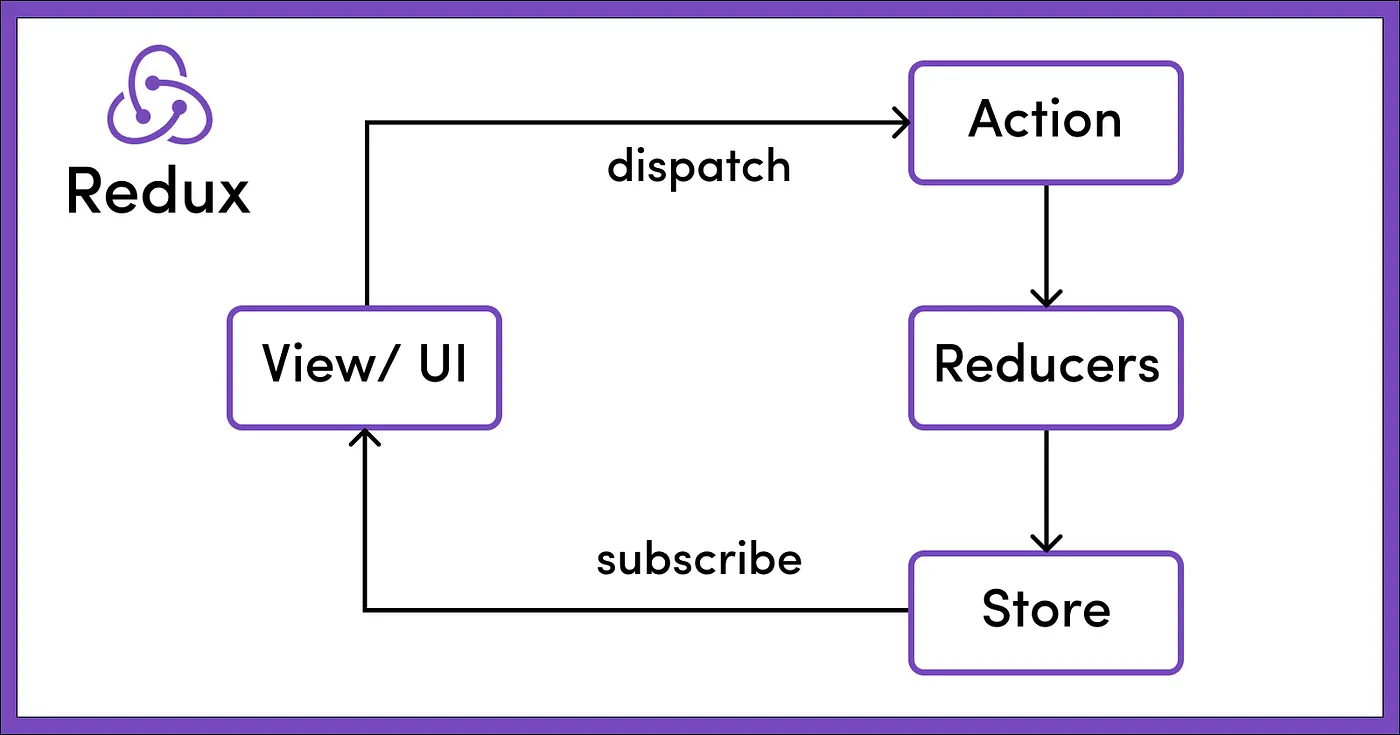
\includegraphics[width=1\textwidth]{redux-lifecycle.png}
  \caption{Redux Datenfluss}
  \label{fig:redux-lifecycle}
\end{figure}

\section{Pinia}

Pinia ist sehr eng gekoppelt mit dem Vue Framework und nutzt dessen Mechanismen der Reaktivität zu Datenhaltung. Das führt dazu, dass Pinia selbst minimal bleibt und die Daten ohne weiteres reaktiv sind. Im Gegensatz zu Redux und NgRx setzt diese Store-Lösung nicht das Flux-Pattern um. Dank dieser Praxis, ist weniger Code nötig um einen Store zu definieren. Außerdem folgt Pinia nicht den Single-Store-Ansatz, bei dem alle Daten in einem zentralen Objekt leben. Sondern sind für Teile der Daten eigenständige Store-Instanzen zuständig. Pinia bietet zwei verschiedene APIs zu Definition von Stores an. In dieser Arbeit wird die \textit{Options API} verwendet. Die Konzepte lassen sich auch auf die \textit{Composition API} übertragen.\cite{piniaDefiningAStore} Die zwei essentiellen Konzepte sind \textit{State} und \textit{Action}.

\subsection{State}

State ist eine Funktion, die ein Objekt zurückgibt. Dieses enthält den Zustand. 

\subsection{Action}

Eine Action ist eine Methode, die den State verändert und in einem \textit{actions} Objekt definiert wird.

\subsection{Definition eines Stores}

Zu Definition eines Stores wird die \textit{defineStore} API genutzt. Als Parameter wird ein eindeutiger Name und eine Beschreibung des Stores in Form eines Objekts übergeben. In dem zweiten Paramter werden die Felder \textit{state} und \textit{actions} definiert.

\begin{lstlisting}
const useUserStore = defineStore('user-store', {
  state: () => {
    user: null
  },
  actions: {
    updateUser(newUser) {
      this.user = newUser
    }
  }
})
\end{lstlisting}

Auf die Felder in dem State-Objekt wird in einer Action mit \textit{this} zugegriffen. Das State-Objekt wird seitens Pinia intern jeder Action gebunden.

\subsection{Interaktion mit dem Store}

Der Store kann in einer belibiegen Vue-Komponente importiert werden. Die Felder des Objekts, das von der state Funktion zurückgegeben wird, werden automatisch zu Feldern des Store Objekts. Genauso werden auch die Methoden des Actions-Objekts auch zu Member des Store Objekts.

\begin{lstlisting}
  const userStore = useUserStore()
  
  // userStore.user
  // userStore.updateUser
\end{lstlisting}

Die State im oberen Beipiel ist reaktiv und kann als \textit{userStore.user} im Template der Komponente referenziert werden. Die Desktrukturierung (destructuring) des Store-Objekts, im oberen Beispiel \textit{userStore}, führt zur Verlust der Reaktivität. Aus diesem Grund wird die Punktnotation empfohlen.\cite{piniaDefiningAStore}

\chapter{Der neue Ansatz} \label{der-neue-ansatz}

\section{Steigende Robustheit durch TypeScript}

% Mehr Projekte nutzen TypeScript => sind bereits was Typing angeht robust
% TypeScript ist auch in fast allen IDEs integriert, also wird fast von jedem genutzt.
TypeScript verfügt, im Gegensatz zu JavaScript, über statische Typisierung. Dank der statischen Typisierung sind statische Typeanalysen und Operationen wie \textit{Go to Definition} und \textit{Go to Implementations} der Entwicklungsumgebungen (IDE) möglich. Diese Eigenschaften reduzieren Fehler im Zusammenhang mit falschen Typen erheblich. Wie in \ref{fig:js-und-ts-nutzung-2018-2024} abgebildet, wird TypeScript von immer mehr Entwicklern genutzt, während die JavaScript Nutzung abnimmt. \ref{fig:js-und-ts-nutzung-2018-2024} beinhaltet die tatsächliche Nutzung von TS nicht. Der TypeScript Compiler (tsc) ist in den meisten modernen IDEs, wie Visual Studio Code und den JetBrains IDEs wie IntelliJ IDEA und WebStorm integriert. Dies führt dazu, dass man auch beim JavaScript Code einige Vorteile von TypeScript bekommt.\cite{typeScriptDocumentary}

\begin{figure}[H]
  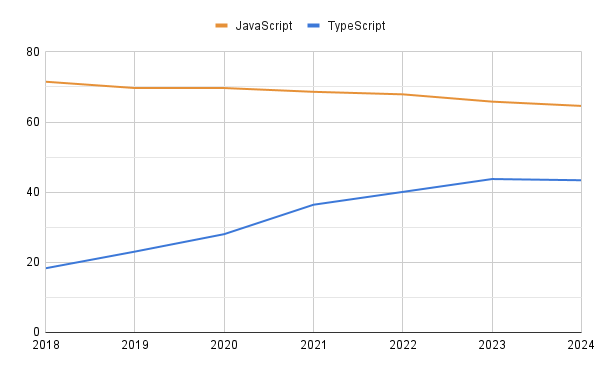
\includegraphics[width=1\textwidth]{js-und-ts-nutzung-2018-2024.png}
  \caption{Prozentuale Nutzung von JavaScript und TypeScript unter professionellen Entwicklern von 2018 bis 2024}
  \label{fig:js-und-ts-nutzung-2018-2024}
\end{figure}

% Um Implementierungsfehler zu vermeiden => Transitions robuster machen

\section {Unzureichende Robustheit in State-Management}

Der TypeScript-Faktor macht Webapplikationen, somit auch State-Management auf Typ-Ebene robuster und weniger fehleranfällig. Allerdings ist es für die Applikation immer noch möglich in einem falschen Zustand zu sein. Gegeben sei ein Redux Store, der für das Speichern einer Liste von \textit{items} zuständig ist. Definiert wird der Store wie folgt:

\begin{lstlisting}
  type FetchAction = {
    type: 'fetch'
  }

  type FetchSuccessfulAction = {
    type: 'fetch-successful',
    payload: Array<any>
  }

  type FetchFailedAction = {
    type: 'fetch-failed',
    payload: Error
  }

  type Action =
    | FetchAction
    | FetchSuccessfulAction
    | FetchFailedAction

  function reducer(
    state = { items: 'not-fetched' }, 
    action: Action
  ) {
    switch (action.type) {
      case 'fetch':
        return {
          ...state,
          items: 'fetching'
        }
      case 'fetch-successful':
        return {
          ...state,
          items: action.payload
        }
      case 'fetch-failed':
        return {
          ...state,
          items: action.payload
        }
      default:
        return state
    }
  }
  
  const store = createStore(reducer)
\end{lstlisting}

Es ist erlaubt, die \textit{FetchSuccessfulAction} Aktion zu versenden, ohne voher die \textit{Fetch} Aktion versendet zu haben. Das heißt: \q{\textit{items} wurden erfolgreich abrufen}, ohne die Anfrage zuvor gemacht zuhaben. Seitens Redux ist das Versenden einer Aktion immer, unbeachtet des aktuellen Zustandes, erlaubt. Dieser Faktor spricht gegen die Nachvollziehbarkeit und gilt für alle populäre SM Lösungen.

\section {Robustere Zustandsübergänge}

% State => Zustand
% Action => Übergang
% Reducer => Übergangsfunktion

Es wird vorgeschlagen den Applikationszustand wie ein Zustand eines DFAs zu behandeln. Im Falle von Redux werden die Aktionen als Übergänge und der Reducer als die Übergangsfunktion eines DFAs gesehen. Restliche Eigenschaften des Quintupels eines DFAs werden hierbei ignoriert.

Um die Übergangsfunktion zu definieren, wird pro Zustand eine \textit{Übergangsliste} aller Aktionen benötigt, die bei diesem Zustand erlaubt sind. Ein Problem hierbei ist allerdings, dass die Identifizierbarkeit der einzelnen Zustände nicht garantiert ist.
Abweichend von DFAs, sind die Zustände in Webapplikationen nicht immer serialisierbar. Nicht serialisierbare Objekte sind nicht immer identifizierbar. Im oberen Beispiel, sind die Zustände \textit{'not-fetched'} und \textit{'fetching'} vom Typ String und somit serialisierbar, allerdings sind die restlichen Zustände nicht serialisierbar (Zustand vom Typ Error und Array<any>). Um dieses Problem zu umgehen, wird eine \textit{identität} Funktion emfohlen, um zwischen verschiedenen Zuständen zu unterscheiden. Sie akzeptiert als Paramter den aktuellen Zustand und gibt ein Boolean zurück.

\begin{lstlisting}
type IdentityFn<S> = (state: S) => boolean
\end{lstlisting}

% ODER SO:
% Sei $S$ die Menge aller Zustände und $B := \{true, false\}$, dann wird die \textit{Konfition Funktion} wie folgt definitiert:
% $f(s) = b | s \in S \land b \in B$

Mit dieser Funktion, kann der Anwender für die Indentifizierbarkeit der Zustände sorgen. Bei JavaScript Klassen, kann der \textit{instanceof} Operator genutzt werden, um auf die Instanz einer Klasse wie \textit{Error} zu prüfen.\cite{jsInstanceofOperator} Desweiteren, können bei Objekten auf eindeutige Eigenschaften, wie die Präzens eines Feldes per \textit{in} Operator geprüft werden.\cite{jsInOperator} Bei Arrays kann die \textit{Array.isArray} Funktion verwendet werden.\cite{jsIsArray} Durch die Kombinition dieser und weiteren Funktionen und Operatoren können weitere Datentypen und Fälle identifiziert werden.

Die \textit{Übergangsliste} lässt sich auch als eine Map wie folgt definieren:

\begin{lstlisting}
type TransitionMap<S extends IdentityFn<S>, A> = Map<S, Array<A>>
\end{lstlisting}

Bei der \textit{Übergangsmap} gilt: \textit{identität} Funktion ist der Schlüssel, während Liste von Aktionen der Wert ist.

In der Übergangsfunktion wird, der Zustandswechsel mit einer \textit{Validierungsfunktion} validiert. Diese prüft mit Hilfe der \textit{Übergangsmap} auf die Gültigkeit eines Übergangs und wirft einen Laufzeitfehler bei ungültigen Aufrufen. Falls der Übergang gültig ist, wirft sie keinen Fehler und der Zustandswechsel kann stattfinden. Der Laufzeitfehler sorgt dafür, dass der ungültige Aufruf berichtet wird und sich nicht zu einem langlebigen Bug entwicklen kann.


\chapter{Vergleich der Ansätze} \label{vergleich}

Der in vorangegangen Kapiteln vorgestellte \acrlong{ac:st}-Ansatz erweitert die interne Funktionsweise einer \acrlong{ac:sm}-Lösung. Er erfordert die zusätzliche Definition einer Transition Map und es werden leicht geänderte APIs dem Benutzer zur Verfügung gestellt. In diesem Kapitel werden die Standard Stores (unveränderte) zu den mit \acrlong{ac:st} verglichen. Es werden die quantifizierbaren Kennzahlen Lines of Code, Bundle Size und Performance untersucht. Außerdem werden die Aspekte \acrlong{ac:dx}, Fehleranfälligkeit, Wartbarkeit und Lesbarkeit analysiert.

\section{Quantifizierbare Aspekte}
\subsection{Lines of Code}

Bei React wurden die .js, .ts, .tsx und bei Vue die .ts und .vue Dateien untersucht. Alle anderen Dateitypen wurden ignoriert, da diese weder für die Geschäftslogik noch für die UI verantwortlich sind.

\begin{table}[!ht]
  \caption{Statische Analyse, Redux und Pinia mit und ohne \acrshort{ac:st}}
  \label{tab:staticAnalysisSTvsNoST}

  \begin{center}
    \begin{tabular}{|c|c|c|c|} 
    \hline
    Dateityp & Anzahl & LOC & Szenario \\ [0.5ex] 
    \hline\hline
    js & 1 & 25 & React ohne ST \\ 
    \hline
    ts & 14 & 256 & React ohne ST \\
    \hline
    tsx & 5 & 187 & React ohne ST \\
    \hline\hline
    js & 1 & 25 & React mit ST \\ 
    \hline
    ts & 17 & 284 & React mit ST \\
    \hline
    tsx & 5 & 187 & React mit ST \\
    \hline\hline
    ts & 5 & 140 & Vue ohne ST \\
    \hline
    vue & 5 & 133 & Vue ohne ST \\
    \hline\hline
    ts & 5 & 172 & Vue mit ST \\
    \hline
    tsx & 5 & 133 & Vue mit ST \\
    \hline
    \end{tabular}
  \end{center}
\end{table}

Der relative Anstieg in \acrshort{ac:loc} beträgt bei React $\sim6\%$ und bei Vue $\sim12\%$. Darüber hinaus beträgt der absolute Anstieg jeweils 28 Lines und 32 Lines. (Siehe Tab. \ref{tab:staticAnalysisSTvsNoST})

\subsection{Bundle Size}

Analysiert wurden die Production Bundles der Applikationen. Diese wurden mit dem Build-Tool Vite erstellt. Alle Applikationen nutzen ausschließlich Client Side Rendering. Daher ist es wichtig, dass die Bundles so klein wie möglich bleiben.

\begin{table}[!ht]
  \caption{Bundle Size Analyse, Redux und Pinia mit und ohne \acrshort{ac:st}}
  \label{tab:bundleSizeAnalysisSTvsNoST}

  \begin{center}
    \begin{tabular}{|c|c|c|} 
    \hline
    Size in kB & Gziped & Szenario \\ [0.5ex]
    \hline\hline
    156,26 & 51,22 & React ohne ST \\
    \hline
    157,24 & 51,54 & React mit ST \\
    \hline
    70,43 & 28,23 & Vue ohne ST \\
    \hline
    71,16 & 28,5 & Vue mit ST \\
    \hline
    \end{tabular}
  \end{center}
\end{table}

Der relative Anstieg beträgt bei React $\sim0,6\%$ und bei Vue $\sim1\%$. Darüber hinaus beträgt der absolute Anstieg jeweils 0,98kB und 0,73kB. Der Anstieg in Bundle Size ist vernachlässigbar. (Siehe Tab. \ref{tab:bundleSizeAnalysisSTvsNoST})

\subsection{Performance}

Um den Unterschied in Performance zu messen, wurde das Testing Tool Playwright verwendet. Mit Hilfe von Playwright wurde ein Szenario definiert. In diesem wurden alle Features der Webseite verwendet, welche Actions in Stores verursachen. Das Szenario wurde pro Applikation 20 Mal ausgeführt. Es lief im Chrome Browser und wurde mit Hilfe des Performance Tabs in den Chrome DevTools analysiert. Es wurden die Mittelwerte für Ausführungszeit in Millisekunden für die Browsertasks Scripting, Painting und Rendering ermittelt.

\begin{table}[!ht]
  \caption{Performance Analyse, Redux und Pinia mit und ohne \acrshort{ac:st}}
  \label{tab:performanceAnalysisSTvsNoST}

  \begin{center}
    \begin{tabular}{|c|c|c|c|c|} 
    \hline
    Task & ms ohne ST & mit ST & Delta & Library \\ [0.5ex]
    \hline\hline
    Scripting & 1.111,45 & 1.121,35 & +0,89\% & Redux \\
    \hline
    Painting & 858,05 & 841,05 & -1,98\% & Redux \\
    \hline
    Rendering & 613,25 & 611,05 & -0,36\% & Redux \\
    \hline
    Scripting & 1.680,15 & 1.677,95 & -0,13\% & Pinia \\
    \hline
    Painting & 777,65 & 763,65 & -1,80\% & Pinia \\
    \hline
    Rendering & 651,65 & 642,9 & -1,34\% & Pinia \\
    \hline
    \end{tabular}
  \end{center}
\end{table}

In allen Browsertasks, ausgenommen Scripting bei React, kann ein Rückgang in der Ausführungszeit beobachtet werden. Allerdings ist der Unterschied vernachlässigbar, da dieser sehr gering ist. Auch der Anstieg im Scripting bei React ist mit 0,89\% ebenfalls vernachlässigbar. (Siehe Tab. \ref{tab:performanceAnalysisSTvsNoST})

Die Gerätespezifikation und Versionen der verwendeten Technologien sind aus der Tabelle \ref{tab:specsAndVersions} im Anhang zu entnehmen.

\section{Qualitative Aspekte}

\subsection{Developer Experience}
Die \acrshort{ac:dx} wird durch die zusätzliche Aufgabe der Definition einer Transition Map beeinflusst. Sie führt zu mehr Code und somit zu zusätzlichem Aufwand.

% TODO mehr Text bei DX ?

\subsection{Fehleranfälligkeit}
Vorausgesetzt, die Transition Map bildet die zulässigen Übergänge vollständig und korrekt ab, kann sich die Applikation nicht in einem unzulässigen Zustand befinden. Obwohl sich hiermit die Fehlerstelle verlagert, ist diese zentral und nicht an vielen Orten verteilt. Falls sich die Applikation in einem falschen Zustand befindet, ist die Transition Map an einem zentralen Ort zu überprüfen, statt die ausgelösten Actions an vielen Orten.

Darüber hinaus bildet die Transition Map die Abläufe in der Applikation ab und kann für eine bessere Nachvollziehbarkeit sorgen. Außerdem ist die Transition Map ein POJO und kann somit ohne weiteres Mocking getestet werden.

\subsection{Lesbarkeit und Wartbarkeit}
Die Lesbarkeit des gesamten Applikationscodes bleibt unverändert, ausgenommen ist die hinzukommende Transition Map. Die Lesbarkeit der Transition Map wird hauptsächlich durch die enthaltenen Identitätsfunktionen beeinflusst. Für diese wird der Einsatz von Pure-Functions mit geringen Abzweigungen und Funktionsaufrufen empfohlen. Wenn dies eingehalten wird, ist die zyklomatische Komplexität gering, was in der Regel eine bessere Lesbarkeit impliziert. Jedoch hängt die Lesbarkeit stark von den Konventionen und dem Code Style des Authors ab. Jede hinzukommende Action oder State muss in der Transition Map berücksichtigt werden. Daher steigt die Wartbarkeit.

% TODO Mehr Text zur Wartbarkeit
\chapter{Beantwortung der Forschungsfragen}
\chapter{Fazit} \label{ch:fazit}

\section{Beantwortung der Forschungsfragen}

Die Hauptgegenstände des \acrlong{ac:st}-Ansatzes sind die Erhöhung der Produktivität des Entwicklers oder der Entwicklerin und das Erkennen von Bugs in frühen Phasen der Entwicklung sowie des Testings im Umgang mit dem Applikationszustand. Um diese Ziele zu erreichen, werden die Zustandsübergänge übersichtlicher an einem zentralen Ort definiert und Laufzeitfehler bei Verstößen geworfen. Die Definition der Zustandsübergänge ist inspiriert von der Übergangsfunktion eines \acrshort{ac:dfa}s. Das liegt an der intuitiven Natur der DFAs und der starken Übereinstimmung im Aufbau mit dem Zustand eines Web-Frontends.

Die drei zentralen Fragen, mit denen sich diese Arbeit beschäftigt, sind:

\begin{enumerate}
  \item Können Bugs, die aufgrund eines falschen Zustands entstehen, mit Hilfe von Strict Transitions reduziert werden?
  \item Steigt oder sinkt die \acrshort{ac:dx} durch die Einführung von Strict Transitions?
  \item Steigt oder sinkt die Lesbarkeit und Wartbarkeit des Codes durch die Einführung von Strict Transitions?
\end{enumerate}

\subsection{Reduzierung von Fehlern}

Damit Fehler im Zustand auf ein Minimum reduziert werden, ist die Definition der zulässigen Zustandsübergänge (Transition Map) erforderlich. Folglich können keine unerlaubten, also undefinierten, Zustandsübergänge stattfinden. Allerdings ist der \acrshort{ac:st}-Ansatz ungeschützt vor fehlerhaften oder unvollständigen Definitionen. Eine Applikation mit einer Transition Map, die die gültigen Geschäftsprozesse und Nutzerinteraktionen nicht widerspiegelt, ist anfällig für Bugs, die im Zusammenhang mit dem State stehen. Diesem Faktor kann die leichte Testbarkeit der Transition Maps entgegenwirken. Trotz der erhöhten Übersichtlichkeit aufgrund des Aufbaus der Transition Maps sind Fehler nach wie vor möglich, auch wenn potenziell in geringerem Umfang. Aus diesem Grund kann keine definitive Antwort auf diese Frage mit den Methoden dieser Arbeit geliefert werden. Eine zutreffendere Antwort sollte auf den Einsatz des \acrshort{ac:st} in realen Applikationen und umfangreiches Testen basieren.

\subsection{Developer Experience}

Auf den ersten Blick kann von einer Verschlechterung der \acrshort{ac:dx} ausgegangen werden. Der Grund hierfür ist die zusätzliche Aufgabe der Definition der Transition Map. Dieser zusätzliche Aufwand kann jedoch potenziell zukünftige Bugs verhindern und somit den Gesamtaufwand für Bugfixes reduzieren. Jedoch kann auch bei diesem Punkt keine definitive Schlussfolgerung mit den Methoden dieser Arbeit gezogen werden.

\subsection{Lesbarkeit und Wartbarkeit}

Die Lesbarkeit und Wartbarkeit der gesamten Applikation bleiben unverändert. Die Lesbarkeit und Wartbarkeit der Transition Map sind hoch, da es sich hierbei um ein einfach testbares \acrshort{ac:pojo} handelt. Jeder dazukommende State muss in der Transition Map ergänzt werden, und genauso muss jeder entfernte State aus der Transition Map gelöscht werden.

\section{Ausblick}

Um die ersten beiden Forschungsfragen endgültig zu beantworten, sollten eine weitreichendere Analyse und Umfragen stattfinden.

Die \acrshort{ac:dx} kann durch Linting Rules, z. B. für ESLint, gesteigert werden. So könnte beispielsweise darauf überprüft werden, dass jede definierte Action in mindestens einer Transition Map referenziert wird. Außerdem könnte mit Hilfe eines Language Servers überprüft werden, dass jeder State mindestens einer Identitätsfunktion zugeordnet werden kann. Ein visueller Editor für die Transition Map könnte die Nachvollziehbarkeit zusätzlich erhöhen und, wenn es um die Geschäftsprozesse geht, als Diskussionshilfe zwischen den Entwicklern und Product-Managern / Product-Ownern dienen.

Im Rahmen dieser Arbeit wurden drei Implementierungen für die Libraries Redux, NgRx und Pinia entwickelt. Diese Auswahl könnte um Libraries wie Zustand und Redux Toolkit erweitert werden.

% Add additional chapters here

%\bibliographystyle{plain}
\bibliographystyle{dinat}
\bibliography{literature}

% Appendix
\appendix
% !TEX root = ./thesis.tex
% appendix example chapter
% @author Thomas Lehmann
%

\chapter{Anhang}

\section{Gerätspezifikation und Versionen der verwendeten Technologien}

\begin{table}[h!]
  \caption{Gerätspezifikation und Versionen der verwendeten Technologien}
  \label{tab:specsAndVersions}
  
  \begin{center}
    \begin{tabular}{ | m{5cm}| m{5cm} | } 
      \hline
      Gerät & Apple Macbook Pro 2023 mit M3 CPU und 24GB Speicher \\ 
      \hline
      Betriebssystem & MacOS 15.3 \\ 
      \hline
      Docker & 27.4.1 \\ 
      \hline
      OrbStack & 1.9.5 \\ 
      \hline
      Nginx & 1.27.3 \\ 
      \hline
      Chrome Canary & 134.0.6994.0 \\ 
      \hline
      Playwright & 1.50.0 \\ 
      \hline
      Node & 20.17.0 \\ 
      \hline
      Vite & 6.0.5 \\ 
      \hline
      React & 18.3.1 \\ 
      \hline
      Redux & 5.0.1 \\ 
      \hline
      React Redux & 9.2.0 \\ 
      \hline
      Vue & 3.5.13 \\ 
      \hline
      Pinia & 2.3.1 \\ 
      \hline
    \end{tabular}
  \end{center}
\end{table}

\section{Beispiele für Implementierung des ST-Ansatzes}

Im Rahmen dieser Arbeit resultierten zwei Implementierung des ST-Ansatzes. Eine für Redux und andere für Pinia. Diese sind im öffentlichen Repository auf Github unter \url{https://github.com/s0h311/strict-transitions} zu finden.

\section{Im Vergleich genutzte Projekte}

Die, im Vergleich genutzten React und Vue Projekte sind im öffentlichen Repository auf Github unter \url{github.com/s0h311/strict-transitions-benchmark} zu finden.

\section{Verwendete Hilfsmittel}
In der Tabelle \ref{tab:tooling} sind die im Rahmen der Bearbeitung des Themas der \IthesisKindDE~verwendeten Werkzeuge und Hilfsmittel aufgelistet.

\begin{table}[h!]
\caption{Verwendete Hilfsmittel und Werkzeuge}
\begin{tabular}{|l|l|}
\hline 
\rowcolor{lightgray} Tool & Verwendung \\
\hline
\LaTeX & Textsatz- und Layout-Werkzeug verwendet zur Erstellung dieses Dokuments \\
\hline
 & \\
\hline
\end{tabular}
\label{tab:tooling}
\end{table}



\IGlossary

\Istatement

\end{document}
